% Created 2024-08-22 Thu 14:01
% Intended LaTeX compiler: xelatex
\documentclass[11pt]{article}
\usepackage{hyperref}
% TIPS
% \substack{a\\b} for multiple lines text





% pdfplots will load xolor automatically without option
\usepackage[dvipsnames]{xcolor}

\usepackage{forest}
% two-line text in node by [two \\ lines]
% \begin{forest} qtree, [..] \end{forest}
\forestset{
  qtree/.style={
    baseline,
    for tree={
      parent anchor=south,
      child anchor=north,
      align=center,
      inner sep=1pt,
    }}}
%\usepackage{flexisym}
% load order of mathtools and mathabx, otherwise conflict overbrace

\usepackage{mathtools}
%\usepackage{fourier}
\usepackage{pgfplots}
\usepackage{amsthm, mathabx,  amsmath, commath}
\usepackage{amsfonts}

\usepackage{empheq}
\usepackage{tikz}
\usetikzlibrary{arrows.meta}
\usepackage[most]{tcolorbox}

\newtheorem{theorem}{Theorem}[section]
\newtheorem{definition}{Definition}[section]
\newtheorem{corollary}{Corollary}[section]
\newtheorem{example}{Example}[section]
\newtheorem{lemma}{Lemma}[section]
\newtheorem{proposition}{Proposition}[section]

\newcommand{\bl}[1] {\boldsymbol{#1}}
\newcommand{\Wt}[1] {\stackrel{\sim}{\smash{#1}\rule{0pt}{1.1ex}}}
\newcommand{\wt}[1] {\widetilde{#1}}


%For boxed texts in align, use Aboxed{}
%otherwise use boxed{}

\DeclareMathSymbol{\widehatsym}{\mathord}{largesymbols}{"62}
\newcommand\lowerwidehatsym{%
  \text{\smash{\raisebox{-1.3ex}{%
    $\widehatsym$}}}}
\newcommand\fixwidehat[1]{%
  \mathchoice
    {\accentset{\displaystyle\lowerwidehatsym}{#1}}
    {\accentset{\textstyle\lowerwidehatsym}{#1}}
    {\accentset{\scriptstyle\lowerwidehatsym}{#1}}
    {\accentset{\scriptscriptstyle\lowerwidehatsym}{#1}}
}

\usepackage{graphicx}
    
% text on arrow for xRightarrow
\makeatletter
%\newcommand{\xRightarrow}[2][]{\ext@arrow 0359\Rightarrowfill@{#1}{#2}}
\makeatother


\def \bx {\boldsymbol{x}}
\def \ba {\boldsymbol{a}}
\def \bI {\boldsymbol{I}}
\def \bt {\boldsymbol{t}}
\def \bb {\boldsymbol{b}}
\def \bA {\boldsymbol{A}}
\def \bX {\boldsymbol{X}}
\def \bu {\boldsymbol{u}}
\def \bS {\boldsymbol{S}}
\def \bZ {\boldsymbol{Z}}
\def \bz {\boldsymbol{z}}
\def \by {\boldsymbol{y}}
\def \bw {\boldsymbol{w}}
\def \bT {\boldsymbol{T}}
\def \bS {\boldsymbol{S}}
\def \bm {\boldsymbol{m}}
\def \bW {\boldsymbol{W}}
\def \bY {\boldsymbol{Y}}
\def \bH {\boldsymbol{H}}
\def \blambda {\boldsymbol{\lambda}}
\def \bPhi {\boldsymbol{\Phi}}
\def \btheta {\boldsymbol{\theta}}
\def \bmu {\boldsymbol{\mu}}
\def \bphi {\boldsymbol{\phi}}
\def \bSigma {\boldsymbol{\Sigma}}
\def \lb {\left\{}
\def \rb {\right\}}
\def \caln {\mathcal{N}}
\def \dissum {\displaystyle\Sigma}
\def \dispro {\displaystyle\prod}
\def \E {\mathbb{E}}
\def \Q {\mathbb{Q}}
\def \V {\mathbb{V}}
\def \R {\mathbb{R}}
\def \calq {\mathcal{Q}}
\def \calg {\mathcal{G}}
\def \caln {\mathcal{N}}
\def \calr {\mathcal{R}}
\def \calm {\mathcal{M}}
\def \calc {\mathcal{C}}
\def \bcup {\bigcup}

\graphicspath{{../../books/}}
\makeindex
\definecolor{mintedbg}{rgb}{0.99,0.99,0.99}
\usepackage[cachedir=\detokenize{~/miscellaneous/trash}]{minted}
\setminted{breaklines,
mathescape,
bgcolor=mintedbg,
fontsize=\footnotesize,
frame=single,
linenos}

%% ox-latex features:
%   !announce-start, !guess-pollyglossia, !guess-babel, !guess-inputenc, caption,
%   underline, image, !announce-end.

\usepackage{capt-of}

\usepackage[normalem]{ulem}

\usepackage{graphicx}

%% end ox-latex features


\author{Paul E. McKenny}
\date{\today}
\title{Is Parallel Programming Hard, And, If So, \\What Can You Do About It?}
\hypersetup{
 pdfauthor={Paul E. McKenny},
 pdftitle={Is Parallel Programming Hard, And, If So, \\What Can You Do About It?},
 pdfkeywords={},
 pdfsubject={},
 pdfcreator={Emacs 31.0.50 (Org mode 9.8-pre)}, 
 pdflang={English}}
\begin{document}

\maketitle
\tableofcontents

\section{Tools of the Trade}
\label{sec:org3bfd19b}
\subsection{POSIX Multiprocessing}
\label{sec:org24bb7d1}
\subsection{Alternatives to POSIX Operations}
\label{sec:org72ed6ef}
\subsection{Accessing Shared Variables}
\label{sec:org89e5972}
\begin{listing}[htbp]
\begin{minted}[]{c}
ptr = global_ptr;
if (ptr != NULL && ptr < high_address)
    do_low(ptr);
\end{minted}
\caption{\label{l4.14}Living Dangerously Early 1990s Style}
\end{listing}

\begin{listing}[htbp]
\begin{minted}[]{c}
if (global_ptr != NULL &&
    global_ptr < high_address)
    do_low(global_ptr);
\end{minted}
\caption{\label{l4.15}C Compilers Can Invent Loads}
\end{listing}
\subsubsection{Shared-Variable Shenanigans}
\label{sec:orgb1549c2}
Given code that does plain loads and stores,the compiler is within its rights to assume that the
affected variables are neither accessed nor modified by any other thread. This assumption allows the
compiler to carry out a large number of transformations, including load tearing, store tearing, load
fusing, store fusing, code reordering, invented loads, invented stores, store-to-load transformations,
and dead- code elimination.

\begin{itemize}
\item \textbf{Load tearing} occurs when the compiler uses multiple load instructions for a single access.
\item \textbf{Store tearing} occurs when the compiler uses multiple store instructions for a single access.
\item \textbf{Load fusing} occurs when the compiler uses the result of a prior load from a given variable instead
of repeating the load.
\begin{listing}[htbp]
\begin{minted}[]{c}
while (!need_to_stop)
    do_something_quickly();
\end{minted}
\caption{\label{l4.16}Inviting Load Fusing}
\end{listing}
\begin{listing}[htbp]
\begin{minted}[]{c}
if (!need_to_stop)
    for (;;) {
        do_something_quickly();
        do_something_quickly();
        do_something_quickly();
        do_something_quickly();
        do_something_quickly();
        do_something_quickly();
        do_something_quickly();
        do_something_quickly();
        do_something_quickly();
        do_something_quickly();
        do_something_quickly();
        do_something_quickly();
        do_something_quickly();
        do_something_quickly();
        do_something_quickly();
        do_something_quickly();
    }
\end{minted}
\caption{\label{l4.17}C Compilers Can Fuse Loads}
\end{listing}
\item \textbf{Store fusing} can occur when the compiler notices a pair of successive stores to a given variable
with no intervening loads from that variable.
\begin{listing}[htbp]
\begin{minted}[]{c}
void shut_it_down(void)
{
    status = SHUTTING_DOWN; /* BUGGY!!! */
    start_shutdown();
    while (!other_task_ready) /* BUGGY!!! */
        continue;
    finish_shutdown();
    status = SHUT_DOWN; /* BUGGY!!! */
    do_something_else();
}

void work_until_shut_down(void)
{
    while (status != SHUTTING_DOWN) /* BUGGY!!! */
        do_more_work();
    other_task_ready = 1; /* BUGGY!!! */
}
\end{minted}
\caption{\label{l4.19}C Compilers Can Fuse Stores}
\end{listing}
\item \textbf{Code reordering}. It might seem futile to prevent the compiler from changing the order of accesses in
cases where the underlying hardware is free to reorder them. However, modern machines have \emph{exact
exceptions} and \emph{exact interrupts}, meaning that any interrupt or exception will appear to have
happened at a specific place in the instruction stream. This means that the handler will see the
effect of all prior instructions, but won't see the effect of any subsequent instructions.
\item \textbf{Invented loads} were illustrated by the code in Listings \ref{l4.14} and \ref{l4.15}, in which the compiler
optimized away a temporary variable, thus loading from a shared variable more often than intended.
\begin{itemize}
\item \textbf{Invented stores}: For example, a compiler emitting code for \texttt{work\_until\_shut\_down()} in Listing
\ref{l4.19} might notice that \texttt{other\_task\_ready} is not accessed by \texttt{do\_more\_work()}, and stored to on
line 16. If \texttt{do\_more\_work()} was a complex inline function, it might be necessary to do a register
spill, in which case one attractive place to use for temporary storage is \texttt{other\_task\_ready}. After
all, there are no accesses to it, so what is the harm?
\end{itemize}
\begin{listing}[htbp]
\begin{minted}[]{c}
if (condition)
    a = 1;
else
    do_a_bunch_of_stuff(&a);
\end{minted}
\caption{\label{l4.20}Inviting an Invented Store}
\end{listing}
\begin{listing}[htbp]
\begin{minted}[]{c}
a = 1;
if (!condition) {
    a = 0;
    do_a_bunch_of_stuff(&a);
}
\end{minted}
\caption{\label{l4.21}Compiler Invents an Invited Store}
\end{listing}
\begin{itemize}
\item \textbf{Store-to-load transformations} can occur when the compiler notices that a plain store might not
actually change the value in memory.
\begin{listing}[htbp]
\begin{minted}[]{c}
r1 = p;
if (unlikely(r1))
    do_something_with(r1);
barrier();
p = NULL;
\end{minted}
\caption{\label{l4.22}Inviting a Store-to-Load Conversion}
\end{listing}
\begin{listing}[htbp]
\begin{minted}[]{c}
r1 = p;
if (unlikely(r1))
    do_something_with(r1);
barrier();
if (p != NULL)
    p = NULL;
\end{minted}
\caption{\label{l4.23}Compiler Converts a Store to a Load}
\end{listing}
\item \textbf{Dead-code elimination}
\end{itemize}
\end{itemize}
\subsubsection{A Volatile Solution}
\label{sec:orga5bce17}
To summarize, the \texttt{volatile} keyword can prevent load tearing and store tearing in cases where the loads
and stores are machine-sized and properly aligned. It can also prevent load fusing, store fusing,
invented loads, and invented stores. However, although it does prevent the compiler from reordering
volatile accesses with each other, it does nothing to prevent the CPU from reordering these accesses.
Furthermore, it does nothing to prevent either compiler or CPU from reordering non-\texttt{volatile} accesses
with each other or with \texttt{volatile} accesses. Preventing these types of reordering requires the techniques described in the next section.
\subsubsection{Assembling the Rest of a Solution}
\label{sec:org41560d4}
\begin{minted}[]{c}
#define barrier() __asm__ __volatile__ ("" : : : "memory")
\end{minted}
In the barrier() macro, the \texttt{\_\_asm\_\_} introduces the asm directive, the \texttt{\_\_volatile\_\_} prevents the
compiler from optimizing the asm away, the empty string specifies that no actual instructions are to
be emitted, and the final \texttt{"memory"} tells the compiler that this do-nothing asm can arbitrarily change
memory. In response, the compiler will avoid moving any memory references across the barrier() macro.
This means that the real-time- destroying loop unrolling shown in Listing \ref{l4.17} can be prevented
by adding \texttt{barrier()} calls as shown on lines 2 and 4 of Listing 4.28.
\wu{
\texttt{barrier()} is for compiler. For hardware, we need \texttt{smp\_mb}
}
\begin{listing}[htbp]
\begin{minted}[]{c}
while (!need_to_stop) {
    barrier();
    do_something_quickly();
    barrier();
}
\end{minted}
\caption{\label{l4.28}Preventing C Compilers From Fusing Loads}
\end{listing}
These two lines of code prevent the compiler from pushing the load from \texttt{need\_to\_stop} into or past
\texttt{do\_something\_quickly()} from either direction.

However, this does nothing to prevent the CPU from reordering the references.
\begin{minted}[]{c}
// arch-arm/arch-arm.h
#define smp_mb()  __asm__ __volatile__("dmb" : : : "memory")

// arch-x86/arch-x86.h
#define smp_mb() __asm__ __volatile__("mfence" : : : "memory")

// arch-ppc64/arch-ppc64.h
#define smp_mb()  __asm__ __volatile__("sync" : : : "memory")

// arch-arm64/arch-arm64.h
#define smp_mb()  __asm__ __volatile__("dmb ish" : : : "memory")
\end{minted}
\section{Deferred Processing}
\label{sec:org1b8666b}
\subsection{Running Example}
\label{sec:orga08b56c}
The value looked up and returned will also be a simple integer, so that the data structure is as shown
in Figure \ref{9.1}, which directs packets with address 42 to interface 1, address 56 to interface 3,
and address 17 to interface 7.

\begin{center}
\includegraphics[width=.99\textwidth]{../images/perfbook/3.png}
\captionof{figure}{\label{9.1}Pre-BSD Packet Routing List}
\end{center}

\begin{listing}[htbp]
\begin{minted}[]{c}
struct route_entry {
    struct cds_list_head re_next;
    unsigned long addr;
    unsigned long iface;
};
CDS_LIST_HEAD(route_list);

unsigned long route_lookup(unsigned long addr)
{
    struct route_entry *rep;
    unsigned long ret;

    cds_list_for_each_entry(rep, &route_list, re_next) {
        if (rep->addr == addr) {
            ret = rep->iface;
            return ret;
        }
    }
    return ULONG_MAX;
}

int route_add(unsigned long addr, unsigned long interface)
{
    struct route_entry *rep;

    rep = malloc(sizeof(*rep));
    if (!rep)
        return -ENOMEM;
    rep->addr = addr;
    rep->iface = interface;
    cds_list_add(&rep->re_next, &route_list);
    return 0;
}

int route_del(unsigned long addr)
{
    struct route_entry *rep;

    cds_list_for_each_entry(rep, &route_list, re_next) {
        if (rep->addr == addr) {
            cds_list_del(&rep->re_next);
            free(rep);
            return 0;
        }
    }
    return -ENOENT;
}
\end{minted}
\caption{\label{l9.1}Sequential Pre-BSD Routing Table}
\end{listing}

Listing \ref{l9.1} (\texttt{route\_seq.c}) shows a simple single-threaded implementation corresponding to Figure \ref{9.1}.
\subsection{Reference Counting}
\label{sec:org2421229}
\label{c9.2}
\begin{listing}[htbp]
\begin{minted}[]{c}
struct route_entry {
    atomic_t re_refcnt;
    struct route_entry *re_next;
    unsigned long addr;
    unsigned long iface;
    int re_freed;
};
struct route_entry route_list;
DEFINE_SPINLOCK(routelock);

static void re_free(struct route_entry *rep)
{
    WRITE_ONCE(rep->re_freed, 1);
    free(rep);
}

unsigned long route_lookup(unsigned long addr)
{
    int old;
    int new;
    struct route_entry *rep;
    struct route_entry **repp;
    unsigned long ret;

retry:
    repp = &route_list.re_next;
    rep = NULL;
    do {
        if (rep && atomic_dec_and_test(&rep->re_refcnt))
            re_free(rep);
        rep = READ_ONCE(*repp);
        if (rep == NULL)
            return ULONG_MAX;
        do {
            if (READ_ONCE(rep->re_freed))
                abort();
            old = atomic_read(&rep->re_refcnt);
            if (old <= 0)
                goto retry;
            new = old + 1;
        } while (atomic_cmpxchg(&rep->re_refcnt,
                                old, new) != old);
        repp = &rep->re_next;
    } while (rep->addr != addr);
    ret = rep->iface;
    if (atomic_dec_and_test(&rep->re_refcnt))
        re_free(rep);
    return ret;
}
\end{minted}
\caption{\label{l9.2}Reference-Counted Pre-BSD Routing Table Lookup (BUGGY)}
\end{listing}

Starting with Listing \ref{l9.2}, line 2 adds the actual reference counter, line 6 adds a \texttt{->re\_freed}
use-after-free check field, line 9 adds the \texttt{routelock} that will be used to synchronize concurrent
updates, and lines 11–15 add \texttt{re\_free()}, which sets \texttt{->re\_freed}, enabling \texttt{route\_lookup()} to check for
use-after-free bugs. In \texttt{route\_lookup()} itself, lines 29–30 release the reference count of the prior
element and free it if the count becomes zero, and lines 34–42 acquire a reference on the new element,
with lines 35 and 36 performing the use-after-free check.

\begin{listing}[htbp]
\begin{minted}[]{c}
int route_add(unsigned long addr, unsigned long interface)
{
    struct route_entry *rep;

    rep = malloc(sizeof(*rep));
    if (!rep)
        return -ENOMEM;
    atomic_set(&rep->re_refcnt, 1);
    rep->addr = addr;
    rep->iface = interface;
    spin_lock(&routelock);
    rep->re_next = route_list.re_next;
    rep->re_freed = 0;
    route_list.re_next = rep;
    spin_unlock(&routelock);
    return 0;
}

int route_del(unsigned long addr)
{
    struct route_entry *rep;
    struct route_entry **repp;

    spin_lock(&routelock);
    repp = &route_list.re_next;
    for (;;) {
        rep = *repp;
        if (rep == NULL)
            break;
        if (rep->addr == addr) {
            *repp = rep->re_next;
            spin_unlock(&routelock);
            if (atomic_dec_and_test(&rep->re_refcnt))
                re_free(rep);
            return 0;
        }
        repp = &rep->re_next;
    }
    spin_unlock(&routelock);
    return -ENOENT;

}
\end{minted}
\caption{\label{l9.3}Reference-Counted Pre-BSD Routing Table Add/Delete (BUGGY)}
\end{listing}

\begin{remark}[]
Why bother with a use-after-free check?

To greatly increase the probability of finding bugs
\end{remark}

In Listing \ref{l9.3}, lines 11, 15, 24, 32, and 39 introduce locking to synchronize concurrent updates.
Line 13 initializes the \texttt{->re\_freed} use-after-free-check field, and finally lines 33–34 invoke
\texttt{re\_free()} if the new value of the reference count is zero.

\begin{remark}[]
Why doesn't \texttt{route\_del()} in Listing \ref{l9.3} use reference counts to protect the traversal to the
element to be freed?

Because the traversal is already protected by the lock, so no additional protection is required.
\end{remark}

\begin{center}
\includegraphics[width=.99\textwidth]{../images/perfbook/4.png}
\captionof{figure}{\label{9.2}Pre-BSD Routing Table Protected by Reference Counting}
\end{center}

Ideal is from Listing \ref{l9.1}. Refcnt performance is abysmal.
\begin{remark}[]
Why the break in the “ideal” line at 224 CPUs in Figure 9.2? Shouldn’t it be a straight line?

The break is due to hyperthreading. On this particular system, the first hardware thread in each core
within a socket have consecutive CPU numbers, followed by the first hardware threads in each core for
the other sockets, and finally followed by the second hardware thread in each core on all the sockets.
On this particular system, CPU numbers 0–27 are the first hardware threads in each of the 28 cores in
the first socket, numbers 28–55 are the first hardware threads in each of the 28 cores in the second
socket, and so on, so that numbers 196–223 are the first hardware threads in each of the 28 cores in
the eighth socket. Then CPU numbers 224–251 are the second hardware threads in each of the 28 cores of
the first socket, numbers 252–279 are the second hardware threads in each of the 28 cores of the
second socket, and so on until numbers 420–447 are the second hardware threads in each of the 28 cores
of the eighth socket.

Why does this matter?

Because the two hardware threads of a given core share resources, and this workload seems to allow a
single hardware thread to consume more than half of the relevant resources within its core. Therefore,
adding the second hardware thread of that core adds less than one might hope. Other workloads might
gain greater benefit from each core’s second hardware thread, but much depends on the details of both
the hardware and the workload.
\end{remark}

One sequence of events leading to the use-after-free bug is as follows, given the list shown in Figure \ref{l9.1}:
\begin{enumerate}
\item Thread A looks up address 42, reaching line 32 of \texttt{route\_lookup()} in Listing \ref{l9.2}. In other
words, Thread A has a pointer to the first element, but has not yet acquired a reference to it.
\item Thread B invokes \texttt{route\_del()} in Listing \ref{l9.2} to delete the route entry for address 42. It
completes successfully, and because this entry’s \texttt{->re\_refcnt} field was equal to the value one, it
invokes \texttt{re\_free()} to set the \texttt{->re\_freed} field and to free the entry.
\item Thread A continues execution of \texttt{route\_lookup()}. Its rep pointer is non-\texttt{NULL}, but line 35 sees that
its \texttt{->re\_freed} field is non-zero, so line 36 invokes \texttt{abort()}
\end{enumerate}
\subsection{Hazard Pointers}
\label{sec:orgeb3ee58}
\label{c9.3}
One way of avoiding problems with concurrent reference counting is to implement the reference counters
inside out, that is, rather than incrementing an integer stored in the data element, instead store a
pointer to that data element in per-CPU (or per-thread) lists. Each element of these lists is called a
\textbf{hazard pointer}.

The value of a given data element’s “virtual reference counter” can then be obtained by counting the
number of hazard pointers referencing that element. Therefore, if that element has been rendered
inaccessible to readers, and there are no longer any hazard pointers referencing it, that element may
safely be freed.

\begin{minted}[]{c}
/* Parameters to the algorithm:
 *  K: Number of hazard pointers per thread.
 *  H: Number of hazard pointers required.
 *  R: Chosen such that R = H + Omega(H).
 */
#define K 2
#define H (K * NR_THREADS)
#define R (100 + 2*H)

/* Must be the first field in the hazard-pointer-protected structure. */
/* It is illegal to nest one such structure inside another. */
typedef struct hazptr_head {
	struct hazptr_head *next;
} hazptr_head_t;

typedef struct hazard_pointer_s {
	void *  __attribute__ ((__aligned__ (CACHE_LINE_SIZE))) p;
} hazard_pointer;

/* Must be dynamically initialized to be an array of size H. */
hazard_pointer *HP;

void hazptr_init(void);
void hazptr_thread_exit(void);
void hazptr_scan();
void hazptr_free_later(hazptr_head_t *);
void hazptr_free(void *ptr); /* supplied by caller. */

#define HAZPTR_POISON 0x8

static hazptr_head_t __thread *rlist;
static unsigned long __thread rcount;
static hazptr_head_t __thread **gplist;
\end{minted}

\begin{listing}[htbp]
\begin{minted}[]{c}
static inline void *_h_t_r_impl(void **p,
                                hazard_pointer *hp)
{
    void *tmp;

    tmp = READ_ONCE(*p);
    if (!tmp || tmp == (void *)HAZPTR_POISON)
        return tmp;
    WRITE_ONCE(hp->p, tmp);
    smp_mb();
    if (tmp == READ_ONCE(*p))
        return tmp;
    return (void *)HAZPTR_POISON;
}

#define hp_try_record(p, hp) _h_t_r_impl((void **)(p), hp)

static inline void *hp_record(void **p,
                              hazard_pointer *hp)
{
    void *tmp;

    do {
        tmp = hp_try_record(p, hp);
    } while (tmp == (void *)HAZPTR_POISON);
    return tmp;
}


static inline void hp_clear(hazard_pointer *hp)
{
    smp_mb();
    WRITE_ONCE(hp->p, NULL);
}
\end{minted}
\caption{\label{l9.4}Hazard-Pointer Recording and Clearing}
\end{listing}

The \texttt{hp\_try\_record()} macro on line 16 is simply a casting wrapper for the \texttt{\_h\_t\_r\_impl()} function, which
attempts to store the pointer referenced by \texttt{p} into the hazard pointer referenced by \texttt{hp}. If successful,
it returns the value of the stored pointer. If it fails due to that pointer being \texttt{NULL}, it returns
\texttt{NULL}. Finally, if it fails due to racing with an update, it returns a special \texttt{HAZPTR\_POISON} token.

\begin{remark}[]
Given that papers on hazard pointers use the bottom bits of each pointer to mark deleted elements,
what is up with \texttt{HAZPTR\_POISON}?
\end{remark}

Line 6 reads the pointer to the object to be protected. If line 8 finds that this pointer was either
\texttt{NULL} or the special \texttt{HAZPTR\_POISON} deleted-object token, it returns the pointer’s value to inform the
caller of the failure. Otherwise, line 9 stores the pointer into the specified hazard pointer, and
line 10 forces full ordering of that store with the reload of the original pointer on line 11. If the
value of the original pointer has not changed, then the hazard pointer protects the pointed-to object,
and in that case, line 12 returns a pointer to that object, which also indicates success to the
caller. Otherwise, if the pointer changed between the two \texttt{READ\_ONCE()} invocations, line 13 indicates
failure. (\wu\{the second read ensures that \texttt{p} is not changed between the read and write\})

The \texttt{hp\_clear()} function is even more straightforward, with an \texttt{smp\_mb()} to force full ordering between
the caller’s uses of the object protected by the hazard pointer and the setting of the hazard pointer
to \texttt{NULL}.

Once a hazard-pointer-protected object has been removed from its linked data structure, so that it is
now inaccessible to future hazard-pointer readers, it is passed to \texttt{hazptr\_free\_later()}, which is shown
on lines 48–56 of Listing \ref{l9.5}. Lines 50 and 51 enqueue the object on a per-thread list rlist and
line 52 counts the object in rcount. If line 53 sees that a sufficiently large number of objects are
now queued, line 54 invokes \texttt{hazptr\_scan()} to attempt to free some of them.

\begin{listing}[htbp]
\begin{minted}[]{c}
int compare(const void *a, const void *b)
{
    return ( *(hazptr_head_t **)a - *(hazptr_head_t **)b );
}

void hazptr_scan()
{
    hazptr_head_t *cur;
    int i;
    hazptr_head_t *tmplist;
    hazptr_head_t **plist = gplist;
    unsigned long psize;

    if (plist == NULL) {
        psize = sizeof(hazptr_head_t *) * K * NR_THREADS;
        plist = (hazptr_head_t **)malloc(psize);
        BUG_ON(!plist);
        gplist = plist;
    }
    smp_mb();
    psize = 0;
    for (i = 0; i < H; i++) {
        uintptr_t hp = (uintptr_t)READ_ONCE(HP[i].p);

        if (!hp)
            continue;
        plist[psize++] = (hazptr_head_t *)(hp & ~0x1UL);

    }
    smp_mb();
    qsort(plist, psize, sizeof(hazptr_head_t *), compare);
    tmplist = rlist;
    rlist = NULL;
    rcount = 0;
    while (tmplist != NULL) {
        cur = tmplist;
        tmplist = tmplist->next;
        if (bsearch(&cur, plist, psize,
                    sizeof(hazptr_head_t *), compare)) {
            cur->next = rlist;
            rlist = cur;
            rcount++;
        } else {
            hazptr_free(cur);
        }
    }
}

void hazptr_free_later(hazptr_head_t *n)
{
    n->next = rlist;
    rlist = n;
    rcount++;
    if (rcount >= R) {
        hazptr_scan();
    }
}
\end{minted}
\caption{\label{l9.5}Hazard-Pointer Scanning and Freeing}
\end{listing}


The \texttt{hazptr\_scan()} function is shown on lines 6–46 of the listing. This function relies on a fixed
maximum number of threads (\texttt{NR\_THREADS}) and a fixed maximum number of hazard pointers per thread (\texttt{K}),
which allows a fixed-size array of hazard pointers to be used. Because any thread might need to scan
the hazard pointers, each thread maintains its own array, which is referenced by the per-thread
variable \texttt{gplist}. If line 14 determines that this thread has not yet allocated its gplist, lines 15–18
carry out the allocation. The memory barrier on line 20 ensures that \uline{all threads see the removal of
all objects by this thread} before lines 22–28 scan all of the hazard pointers, accumulating non-\texttt{NULL}
pointers into the \texttt{plist} array and counting them in \texttt{psize}. The memory barrier on line 29 ensures that
the reads of the hazard pointers happen before any objects are freed. Line 30 then sorts this array to
enable use of binary search below.

Lines 31 and 32 remove all elements from this thread’s list of to-be-freed objects, placing them on
the local tmplist and line 33 zeroes the count. Each pass through the loop spanning lines 34–45
processes each of the to-be-freed objects. Lines 35 and 36 remove the first object from tmplist, and
if lines 37 and 38 determine that there is a hazard pointer protecting this object, lines 39–41 place
it back onto rlist. Otherwise, line 43 frees the object.

The Pre-BSD routing example can use hazard pointers as shown in Listing \ref{l9.6} for data structures
and \texttt{route\_lookup()}, and in Listing 9.7 for \texttt{route\_add()} and \texttt{route\_del()} (\texttt{route\_hazptr.c}). As with
reference counting, the hazard-pointers implementation is quite similar to the sequential algorithm
shown in Listing \ref{l9.1}, so only differences will be discussed.
\begin{listing}[htbp]
\begin{minted}[]{c}
struct route_entry {
    struct hazptr_head hh;
    struct route_entry *re_next;
    unsigned long addr;
    unsigned long iface;
    int re_freed;
};
struct route_entry route_list;
DEFINE_SPINLOCK(routelock);
hazard_pointer __thread *my_hazptr;

unsigned long route_lookup(unsigned long addr)
{
    int offset = 0;
    struct route_entry *rep;
    struct route_entry **repp;

retry:
    repp = &route_list.re_next;
    do {
        rep = hp_try_record(repp, &my_hazptr[offset]);
        if (!rep)
            return ULONG_MAX;
        if ((uintptr_t)rep == HAZPTR_POISON)
            goto retry;
        repp = &rep->re_next;
    } while (rep->addr != addr);
    if (READ_ONCE(rep->re_freed))
        abort();
    return rep->iface;
}
\end{minted}
\caption{\label{l9.6}Hazard-Pointer Pre-BSD Routing Table Lookup}
\end{listing}

Starting with Listing \ref{l9.6}, line 2 shows the \texttt{->hh} field used to queue objects pending
hazard-pointer free, line 6 shows the \texttt{->re\_freed} field used to detect use-after-free bugs, and line 21
invokes \texttt{hp\_try\_record()} to attempt to acquire a hazard pointer. If the return value is \texttt{NULL}, line 23
returns a not-found indication to the caller. If the call to \texttt{hp\_try\_record()} raced with deletion, line
25 branches back to line 18’s retry to re-traverse the list from the beginning. The do–while loop
falls through when the desired element is located, but if this element has already been freed, line 29
terminates the program. Otherwise, the element’s \texttt{->iface} field is returned to the caller.

Note that line 21 invokes \texttt{hp\_try\_record()} rather than the easier-to-use \texttt{hp\_record()}, restarting the
full search upon \texttt{hp\_try\_record()} failure. And such restarting is absolutely required for correctness.
To see this, consider a hazard-pointer-protected linked list containing elements A, B, and C that is
subjected to the following sequence of events:
\begin{enumerate}
\item Thread 0 stores a hazard pointer to element B (having presumably traversed to element B from element A).
\item Thread 1 removes element B from the list, which sets the pointer from element B to element C to the
special \texttt{HAZPTR\_POISON} value in order to mark the deletion. Because Thread 0 has a hazard pointer to
element B, it cannot yet be freed.
\item Thread 1 removes element C from the list. Because there are no hazard pointers referencing element
C, it is immediately freed.
\item Thread 0 attempts to acquire a hazard pointer to now-removed element B’s successor, but
\texttt{hp\_try\_record()} returns the \texttt{HAZPTR\_POISON} value, forcing the caller to restart its traversal from
the beginning of the list.
\end{enumerate}

Therefore, hazard-pointer readers must typically restart the full traversal in the face of a
concurrent deletion.

These hazard-pointer restrictions result in great benefits to readers, courtesy of the fact that the
hazard pointers are stored local to each CPU or thread, which in turn allows traversals to be carried
out without any writes to the data structures being traversed.

\begin{listing}[htbp]
\begin{minted}[]{c}
int route_add(unsigned long addr, unsigned long interface)
{
    struct route_entry *rep;

    rep = malloc(sizeof(*rep));
    if (!rep)
        return -ENOMEM;
    rep->addr = addr;
    rep->iface = interface;
    rep->re_freed = 0;
    spin_lock(&routelock);
    rep->re_next = route_list.re_next;
    route_list.re_next = rep;
    spin_unlock(&routelock);
    return 0;
}


int route_del(unsigned long addr)
{
    struct route_entry *rep;
    struct route_entry **repp;

    spin_lock(&routelock);
    repp = &route_list.re_next;
    for (;;) {
        rep = *repp;
        if (rep == NULL)
            break;
        if (rep->addr == addr) {
            *repp = rep->re_next;
            rep->re_next = (struct route_entry *)HAZPTR_POISON;
            spin_unlock(&routelock);
            hazptr_free_later(&rep->hh);
            return 0;
        }
        repp = &rep->re_next;
    }
    spin_unlock(&routelock);
    return -ENOENT;
}
\end{minted}
\caption{\label{l9.7}Hazard-Pointer Pre-BSD Routing Table Add/Delete}
\end{listing}

\begin{center}
\includegraphics[width=.88\textwidth]{../images/perfbook/56.png}
\captionof{figure}{\label{9.3}Pre-BSD Routing Table Protected by Hazard Pointers}
\end{center}

\begin{remark}[]
\begin{itemize}
\item Figure \ref{9.3} shows no sign of hyperthread-induced flattening at 224 threads. Why is that?

Modern microprocessors are complicated beasts, so signif- icant skepticism is appropriate for any
simple answer. That aside, the most likely reason is the full memory barriers required by
hazard-pointers readers. Any delays resulting from those memory barriers would make time available
to the other hardware thread sharing the core, resulting in greater scalability at the expense of
per-hardware-thread performance.
\item \cite{10.1145/2483852.2483867} shows that hazard pointers have near-ideal performance. Whatever
happened in Figure \ref{9.3}?
\end{itemize}
\end{remark}
\subsection{Sequence Locks}
\label{sec:org7468933}
\label{c9.4}
The key component of sequence locking is the sequence number, which has an even value in the absence
of updaters and an odd value if there is an update in progress. Readers can then snapshot the value
before and after each access. If either snapshot has an odd value, or if the two snapshots differ,
there has been a concurrent update, and the reader must discard the results of the access and then
retry it. Readers therefore use the \texttt{read\_seqbegin()} and \texttt{read\_seqretry()} functions shown in Listing \ref{l9.8}
when accessing data protected by a sequence lock. Writers must increment the value before and after
each update, and only one writer is permitted at a given time. Writers therefore use the
\texttt{write\_seqlock()} and \texttt{write\_sequnlock()} functions shown in Listing \ref{l9.9} when updating data protected
by a sequence lock.

\begin{listing}[htbp]
\begin{minted}[]{c}
do {
    seq = read_seqbegin(&test_seqlock);
    /* read-side access. */
} while (read_seqretry(&test_seqlock, seq));
\end{minted}
\caption{\label{l9.8}Sequence-Locking Reader}
\end{listing}

\begin{listing}[htbp]
\begin{minted}[]{c}
write_seqlock(&test_seqlock);
/* Update */
write_sequnlock(&test_seqlock);
\end{minted}
\caption{\label{l9.9}Sequence-Locking Writer}
\end{listing}

\begin{listing}[htbp]
\begin{minted}[]{c}
typedef struct {
    unsigned long seq;
    spinlock_t lock;
} seqlock_t;

static inline void seqlock_init(seqlock_t *slp)
{
    slp->seq = 0;
    spin_lock_init(&slp->lock);
}

static inline unsigned long read_seqbegin(seqlock_t *slp)
{
    unsigned long s;

    s = READ_ONCE(slp->seq);
    smp_mb();
    return s & ~0x1UL;
}

static inline int read_seqretry(seqlock_t *slp,
                                unsigned long oldseq)
{
    unsigned long s;

    smp_mb();
    s = READ_ONCE(slp->seq);
    return s != oldseq;
}


static inline void write_seqlock(seqlock_t *slp)
{
    spin_lock(&slp->lock);
    ++slp->seq;
    smp_mb();
}
static inline void write_sequnlock(seqlock_t *slp)
{
    smp_mb();
    ++slp->seq;
    spin_unlock(&slp->lock);
}
\end{minted}
\caption{\label{l9.10}Sequence-Locking Implementation}
\end{listing}

\begin{remark}[]
Why not have \texttt{read\_seqbegin()} in \ref{l9.10} check for the low-order bit being set, and retry internally,
rather than allowing a doomed read to start?

That would be a legitimate implementation. However, if the workload is read-mostly, it would likely
increase the overhead of the common-case successful read, which could be counter-productive. However,
given a sufficiently large fraction of updates and sufficiently high-overhead readers, having the
check internal to \texttt{read\_seqbegin()} might be preferable
\end{remark}

Line 17 orders this snapshot before the caller's critical section. Line 26 orders the caller's prior
critical section before line 27's fetch.
\begin{remark}[]
\begin{itemize}
\item Why is the \texttt{smp\_mb()} on line 26 of Listing \ref{l9.10} needed?

If it was omitted, both the compiler and the CPU would be within their rights to move the critical
section Preceding the call to \texttt{read\_seqretry()} down below this function. This would prevent the
sequence lock from protecting the critical section. The \texttt{smp\_mb()} primitive prevents such reordering.
\item Can’t weaker memory barriers be used in the code in Listing \ref{l9.10}?
\item Why isn’t seq on line 2 of Listing \ref{l9.10} unsigned rather than \texttt{unsigned long}? After all, if
\texttt{unsigned} is good enough for the Linux kernel, shouldn’t it be good enough for everyone?

Overflow issue, 32 bit can be easily overflowed
\end{itemize}
\end{remark}

\begin{listing}[htbp]
\begin{minted}[]{c}
struct route_entry {
    struct route_entry *re_next;
    unsigned long addr;
    unsigned long iface;
    int re_freed;
};

struct route_entry route_list;
DEFINE_SEQ_LOCK(sl);

unsigned long route_lookup(unsigned long addr)
{
    struct route_entry *rep;
    struct route_entry **repp;
    unsigned long ret;
    unsigned long s;

retry:
    s = read_seqbegin(&sl);
    repp = &route_list.re_next;
    do {
        rep = READ_ONCE(*repp);
        if (rep == NULL) {
            if (read_seqretry(&sl, s))
                goto retry;
            return ULONG_MAX;
        }
        repp = &rep->re_next;
    } while (rep->addr != addr);
    if (READ_ONCE(rep->re_freed))
        abort();
    ret = rep->iface;
    if (read_seqretry(&sl, s))
        goto retry;
    return ret;
}
\end{minted}
\caption{\label{l9.11}Sequence-Locked Pre-BSD Routing Table Lookup (BUGGY)}
\end{listing}

It suffers use-after-free failures. The problem is that the reader might encounter a segmentation
violation due to accessing an already-freed structure before \texttt{read\_seqretry()} has a chance to warn of
the concurrent update.

\begin{remark}[]
Can this bug be fixed? In other words, can you use sequence locks as the only synchronization
mechanism protecting a linked list supporting concurrent addition, deletion, and lookup?

One trivial way of accomplishing this is to surround all accesses, including the read-only accesses,
with \texttt{write\_ seqlock()} and \texttt{write\_sequnlock()}. Of course, this solution also prohibits all read-side
parallelism, resulting in massive lock contention, and furthermore could just as easily be implemented using
simple locking.

If you do come up with a solution that uses \texttt{read\_ seqbegin()} and \texttt{read\_seqretry()} to protect read-side
accesses, make sure that you correctly handle the following sequence of events:
\begin{enumerate}
\item CPU 0 is traversing the linked list, and picks up a pointer to list element A.
\item CPU 1 removes element A from the list and frees it.
\item CPU 2 allocates an unrelated data structure, and gets the memory formerly occupied by element A. In
this unrelated data structure, the memory previously used for element A’s ->next pointer is now
occupied by a floating-point number.
\item CPU 0 picks up what used to be element A’s -> next pointer, gets random bits, and therefore gets a
segmentation fault.
\end{enumerate}

One way to protect against this sort of problem requires use of “type-safe memory”. Roughly similar
solutions are possible using the hazard pointers. But in either case, you would be using some other
synchronization mechanism in addition to sequence locks!
\end{remark}

\begin{center}
\includegraphics[width=.8\textwidth]{../images/perfbook/5.png}
\captionof{figure}{\label{}Pre-BSD Routing Table Protected by Sequence Locking}
\end{center}
\subsection{Read-Copy Update (RCU)}
\label{sec:org6b5648c}
\label{c9.5}
All of the mechanisms discussed in the preceding sections used one of a number of approaches to defer
specific actions until they may be carried out safely. The reference counters discussed in Section \ref{c9.2}
use explicit counters to defer actions that could disturb readers, which results in read-side
contention and thus poor scalability. The hazard pointers covered by Section \ref{c9.3} uses implicit
counters in the guise of per-thread lists of pointer. This avoids read-side contention, but requires
readers to do stores and conditional branches, as well as either full memory barriers in read-side
primitives or real-time-unfriendly inter-processor interrupts in update-side primitives. The sequence
lock presented in Section \ref{c9.4} also avoids read-side contention, but does not protect pointer
traversals and, like hazard pointers, requires either full memory barriers in read-side primitives, or
inter-processor interrupts in update-side primitives.
\subsubsection{Introduction to RCU}
\label{sec:org5f4a78d}
To minimize implementability concerns, we focus on a minimal data structure, which consists of a
single global pointer that is either \texttt{NULL} or references a single structure.
\begin{center}
\includegraphics[width=.8\textwidth]{../images/perfbook/6.png}
\captionof{figure}{\label{9.6}Insertion With Concurrent Readers}
\end{center}

\begin{center}
\includegraphics[width=.8\textwidth]{../images/perfbook/7.png}
\captionof{figure}{\label{9.7}Insertion With Concurrent Readers}
\end{center}

\begin{remark}[]
\begin{itemize}
\item Why does Figure \ref{9.7} use \texttt{smp\_store\_release()} given that it is storing a \texttt{NULL} pointer? Wouldn’t
\texttt{WRITE\_ONCE()} work just as well in this case, given that there is no structure initialization to
order against the store of the \texttt{NULL} pointer?

Yes, it would.

Because a \texttt{NULL} pointer is being assigned, there is nothing to order against, so there is no need for
\texttt{smp\_store\_ release()}. In contrast, when assigning a non-\texttt{NULL} pointer, it is necessary to use
\texttt{smp\_store\_release()} in order to ensure that initialization of the pointed-to structure is carried
out before assignment of the pointer.

In short, \texttt{WRITE\_ONCE()} would work, and would save a little bit of CPU time on some architectures.
However, as we will see, software-engineering concerns will motivate use of a special
\texttt{rcu\_assign\_pointer()} that is quite similar to \texttt{smp\_store\_release()}.
\item Readers running concurrently with each other and with the procedure outlined in Figure \ref{9.7} can
disagree on the value of \texttt{gptr}. Isn’t that just a wee bit problematic???

Not necessarily.

As hinted at in Sections 3.2.3 and 3.3, speed-of-light delays mean that a computer’s data is always stale com- pared to whatever external reality that data is intended to model.

Real-world algorithms therefore absolutely must tolerate inconsistancies between external reality
and the in-computer data reflecting that reality. Many of those algorithms are also able to tolerate
some degree of inconsistency within the in-computer data. Section 10.3.4 discusses this point in
more detail.

Please note that this need to tolerate inconsistent and stale data is not limited to RCU. It also
applies to reference counting, hazard pointers, sequence locks, and even to some locking use cases.
For example, if you compute some quantity while holding a lock, but use that quantity after
releasing that lock, you might well be using stale data. After all, the data that quantity is based
on might change arbitrarily as soon as the lock is released.

So yes, RCU readers can see stale and inconsistent data, but no, this is not necessarily
problematic. And, when needed, there are RCU usage patterns that avoid both staleness and
inconsistency
\end{itemize}
\end{remark}
\section{Appendices\hfill{}\textsc{ignore}}
\label{sec:org109ef1f}
\appendix
\subsection{Why Memory Barriers}
\label{sec:orgd9e569f}
\subsubsection{Cache Structure}
\label{sec:org210a0d8}
\begin{center}
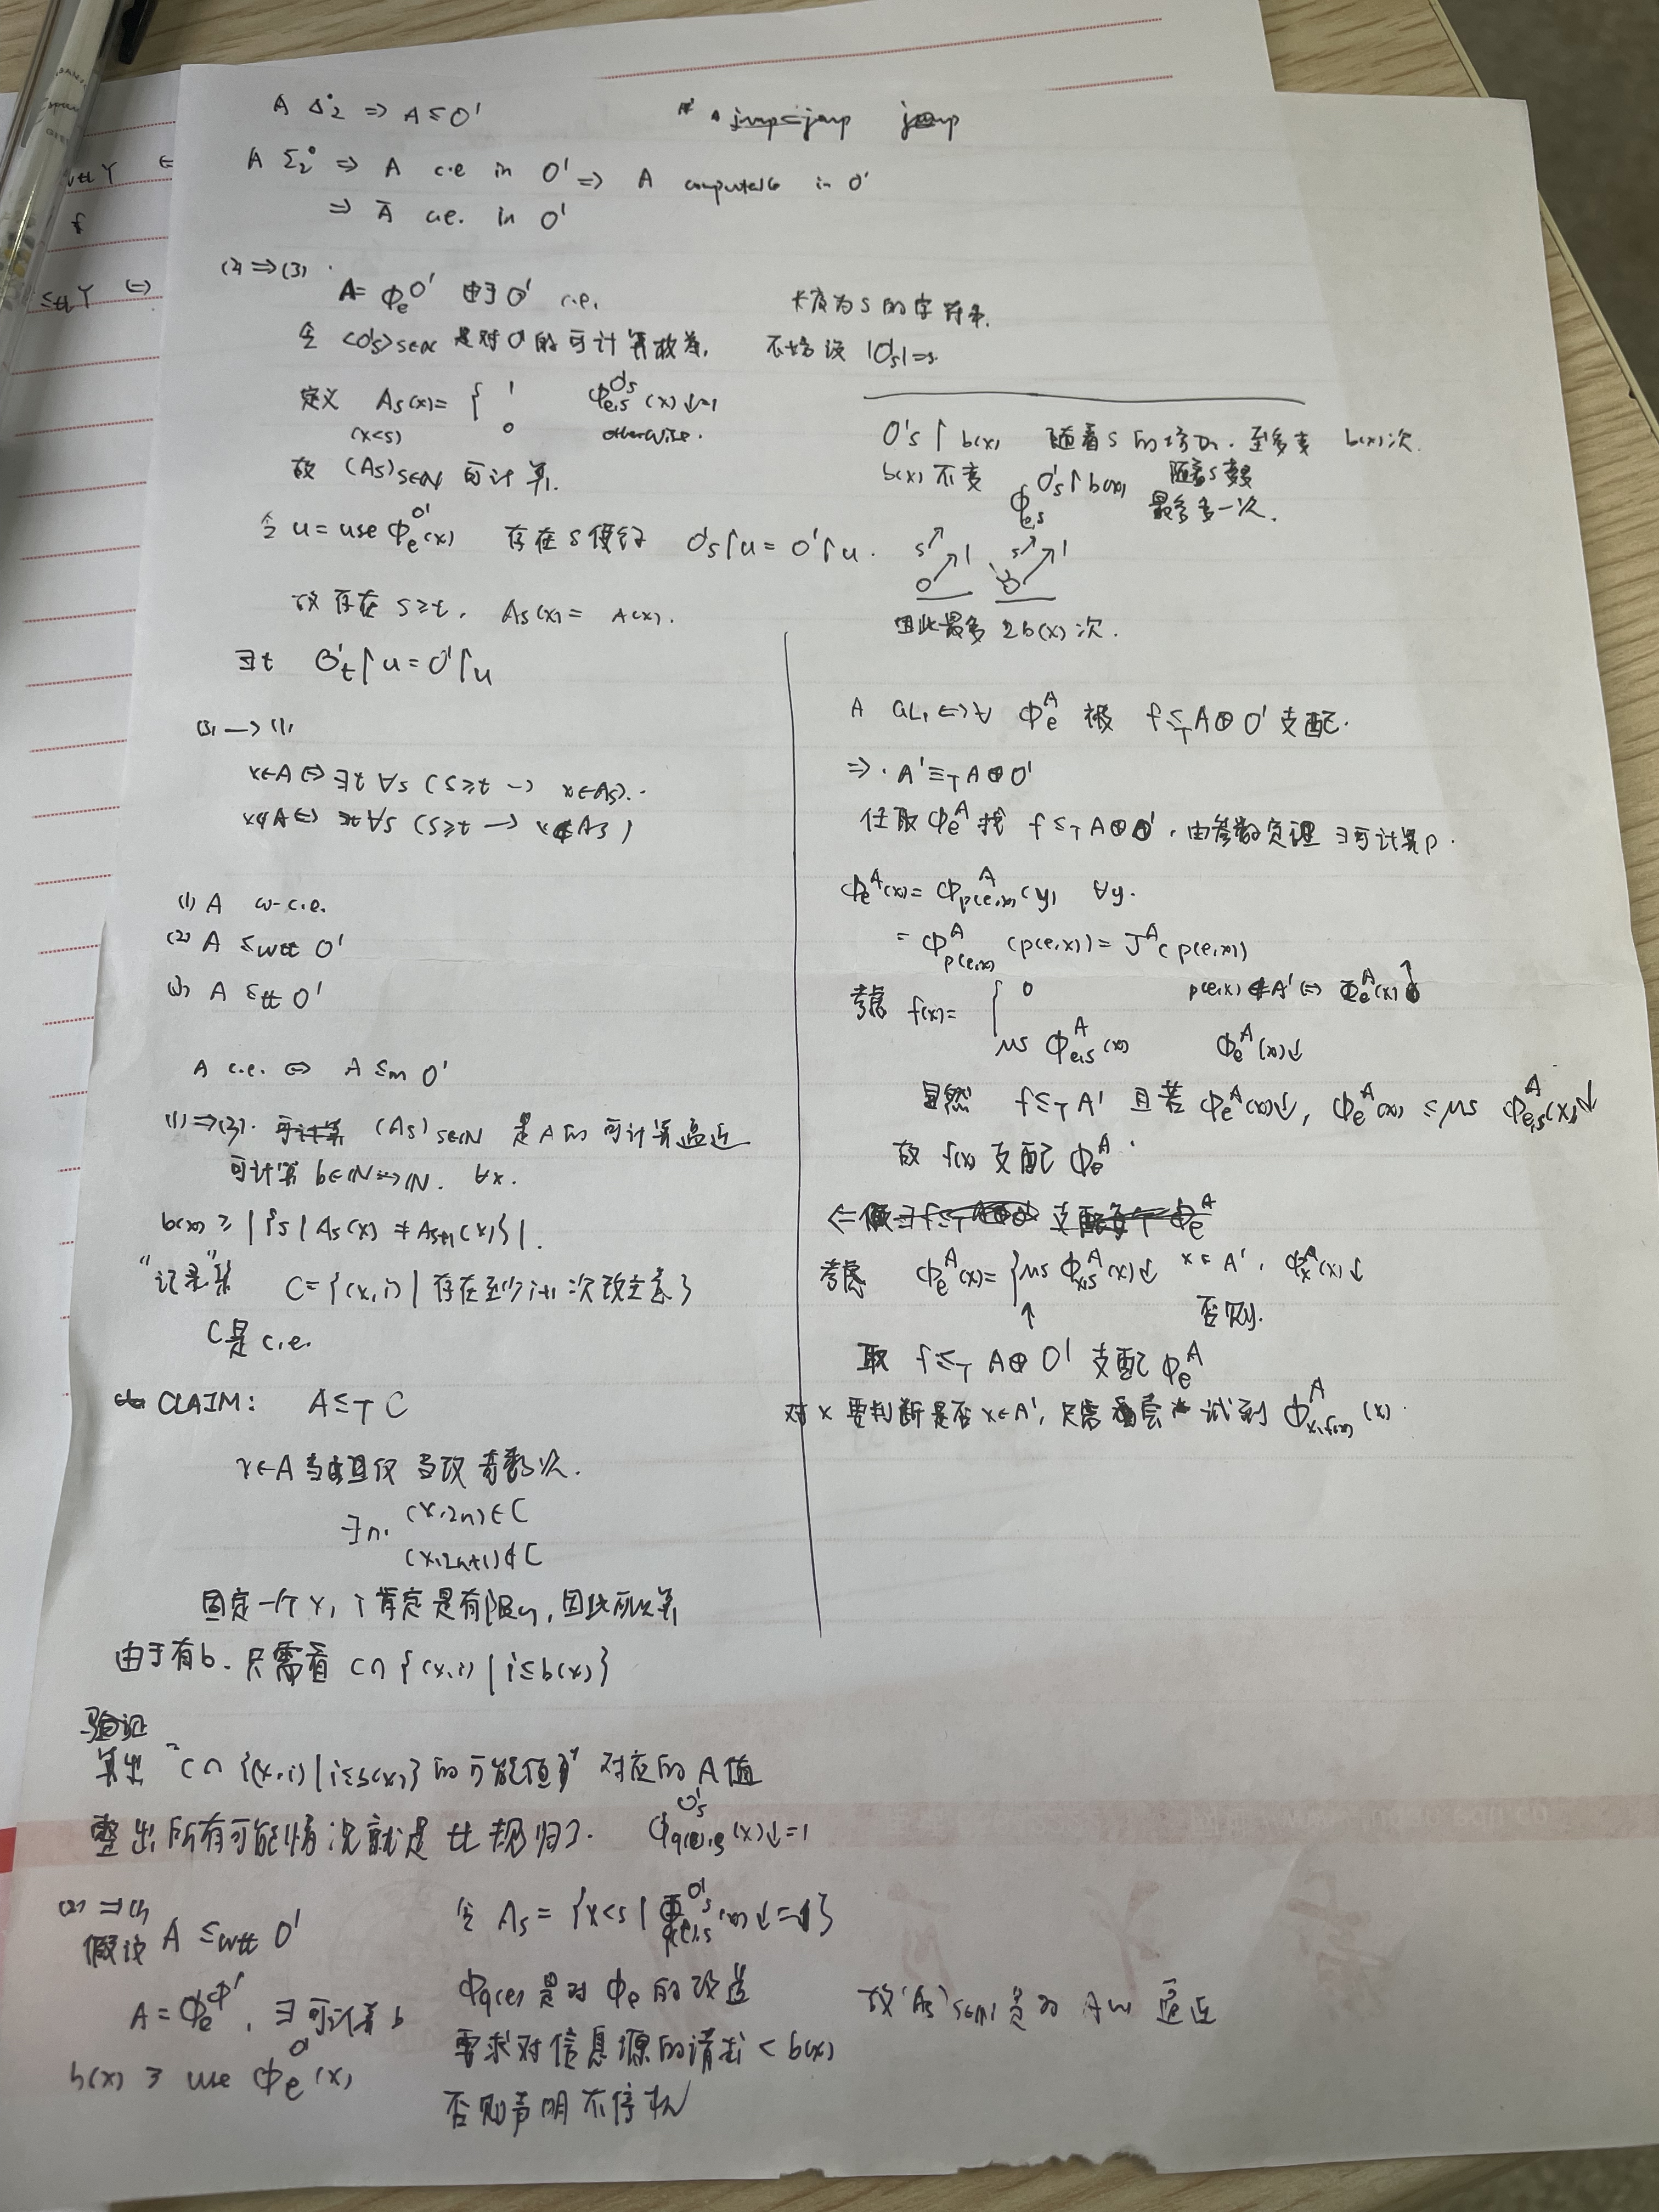
\includegraphics[width=.7\textwidth]{../images/perfbook/1.png}
\captionof{figure}{\label{}Modern Computer System Cache Structure}
\end{center}

Data flows among the CPUs’ caches and memory in fixed-length blocks called “cache lines”, which
are normally a power of two in size, ranging from 16 to 256 bytes. When a given data item is
first accessed by a given CPU, it will be absent from that CPU’s cache, meaning that a “cache
miss” (or, more specifically, a “startup” or “warmup” cache miss) has occurred. The cache miss
means that the CPU will have to wait (or be “stalled”) for hundreds of cycles while the item is
fetched from memory. However, the item will be loaded into that CPU’s cache, so that subsequent
accesses will find it in the cache and therefore run at full speed.

\begin{center}
\includegraphics[width=.8\textwidth]{../images/perfbook/2.png}
\captionof{figure}{\label{}CPU Cache Structure}
\end{center}

This cache has sixteen “sets” and two “ways” for a total of 32 “lines”, each entry containing a
single 256-byte “cache line”, which is a 256-byte-aligned block of memory.

Each box corresponds to a cache entry, which can contain a 256-byte cache line. Since the cache
lines must be 256-byte aligned, the low eight bits of each address are zero, and the choice of
hardware hash function means that the next-higher four bits match the hash line number.

What happens when it does a write? Because it is important that all CPUs agree on the value of a
given data item, before a given CPU writes to that data item, it must first cause it to be
removed, or “invalidated”, from other CPUs’ caches. Once this invalidation has completed, the
CPU may safely modify the data item. If the data item was present in this CPU’s cache, but was
read-only, this process is termed a “write miss”. Once a given CPU has completed invalidating a
given data item from other CPUs’ caches, that CPU may repeatedly write (and read) that data
item.

Later, if one of the other CPUs attempts to access the data item, it will incur a cache miss,
this time because the first CPU invalidated the item in order to write to it. This type of cache
miss is termed a “communication miss”, since it is usually due to several CPUs using the data
items to communicate (for example, a lock is a data item that is used to communicate among CPUs
using a mutual-exclusion algorithm).

Clearly, much care must be taken to ensure that all CPUs maintain a coherent view of the data.
With all this fetching, invalidating, and writing, it is easy to imagine data being lost or
(perhaps worse) different CPUs having conflicting values for the same data item in their
respective caches.
\subsubsection{Cache-Coherence Protocols}
\label{sec:orgf9912ce}
\begin{enumerate}
\item MESI States
\label{sec:org6f3faef}
MESI stands for ``modified'', ``exclusive'', ``shared'', and ``invalid'', the four states a given cache
line can take on using this protocol.
\end{enumerate}
\end{document}
